\begin{center}
	\underline{\Large\scshape\bfseries \dytema}
\end{center}
%\markright{INFORME LABORATORIO Nº 05}
%-------------------------------------------------------------------------------------------
\section{Objetivos}
\begin{enumerate}[label=\itemcirccz{azzul}{\arabic*},itemsep=2pt]
	\item Estudiar y analizar el movimiento de un resorte vertical oscilante y un péndulo simple.
	\item Investigar y descubrir la relacion del periodo y la masa, la relación de la longitud del péndulo y el periodo.
	\item Determinar la aceleración de la gravedad en Ayacucho.
\end{enumerate}
%-------------------------------------------------------------------------------------------
\section{Materiales y equipos}
\begin{itemize}[label=\textbf{$\bullet$},itemsep=2pt]
	\item Soportes universales con base triangular.
	\item Juego de pesas.
	\item Regla graduada.
	\item Cronómetro.
\end{itemize}

\begin{multicols}{2}
	\begin{figure}[H]
		\centering
		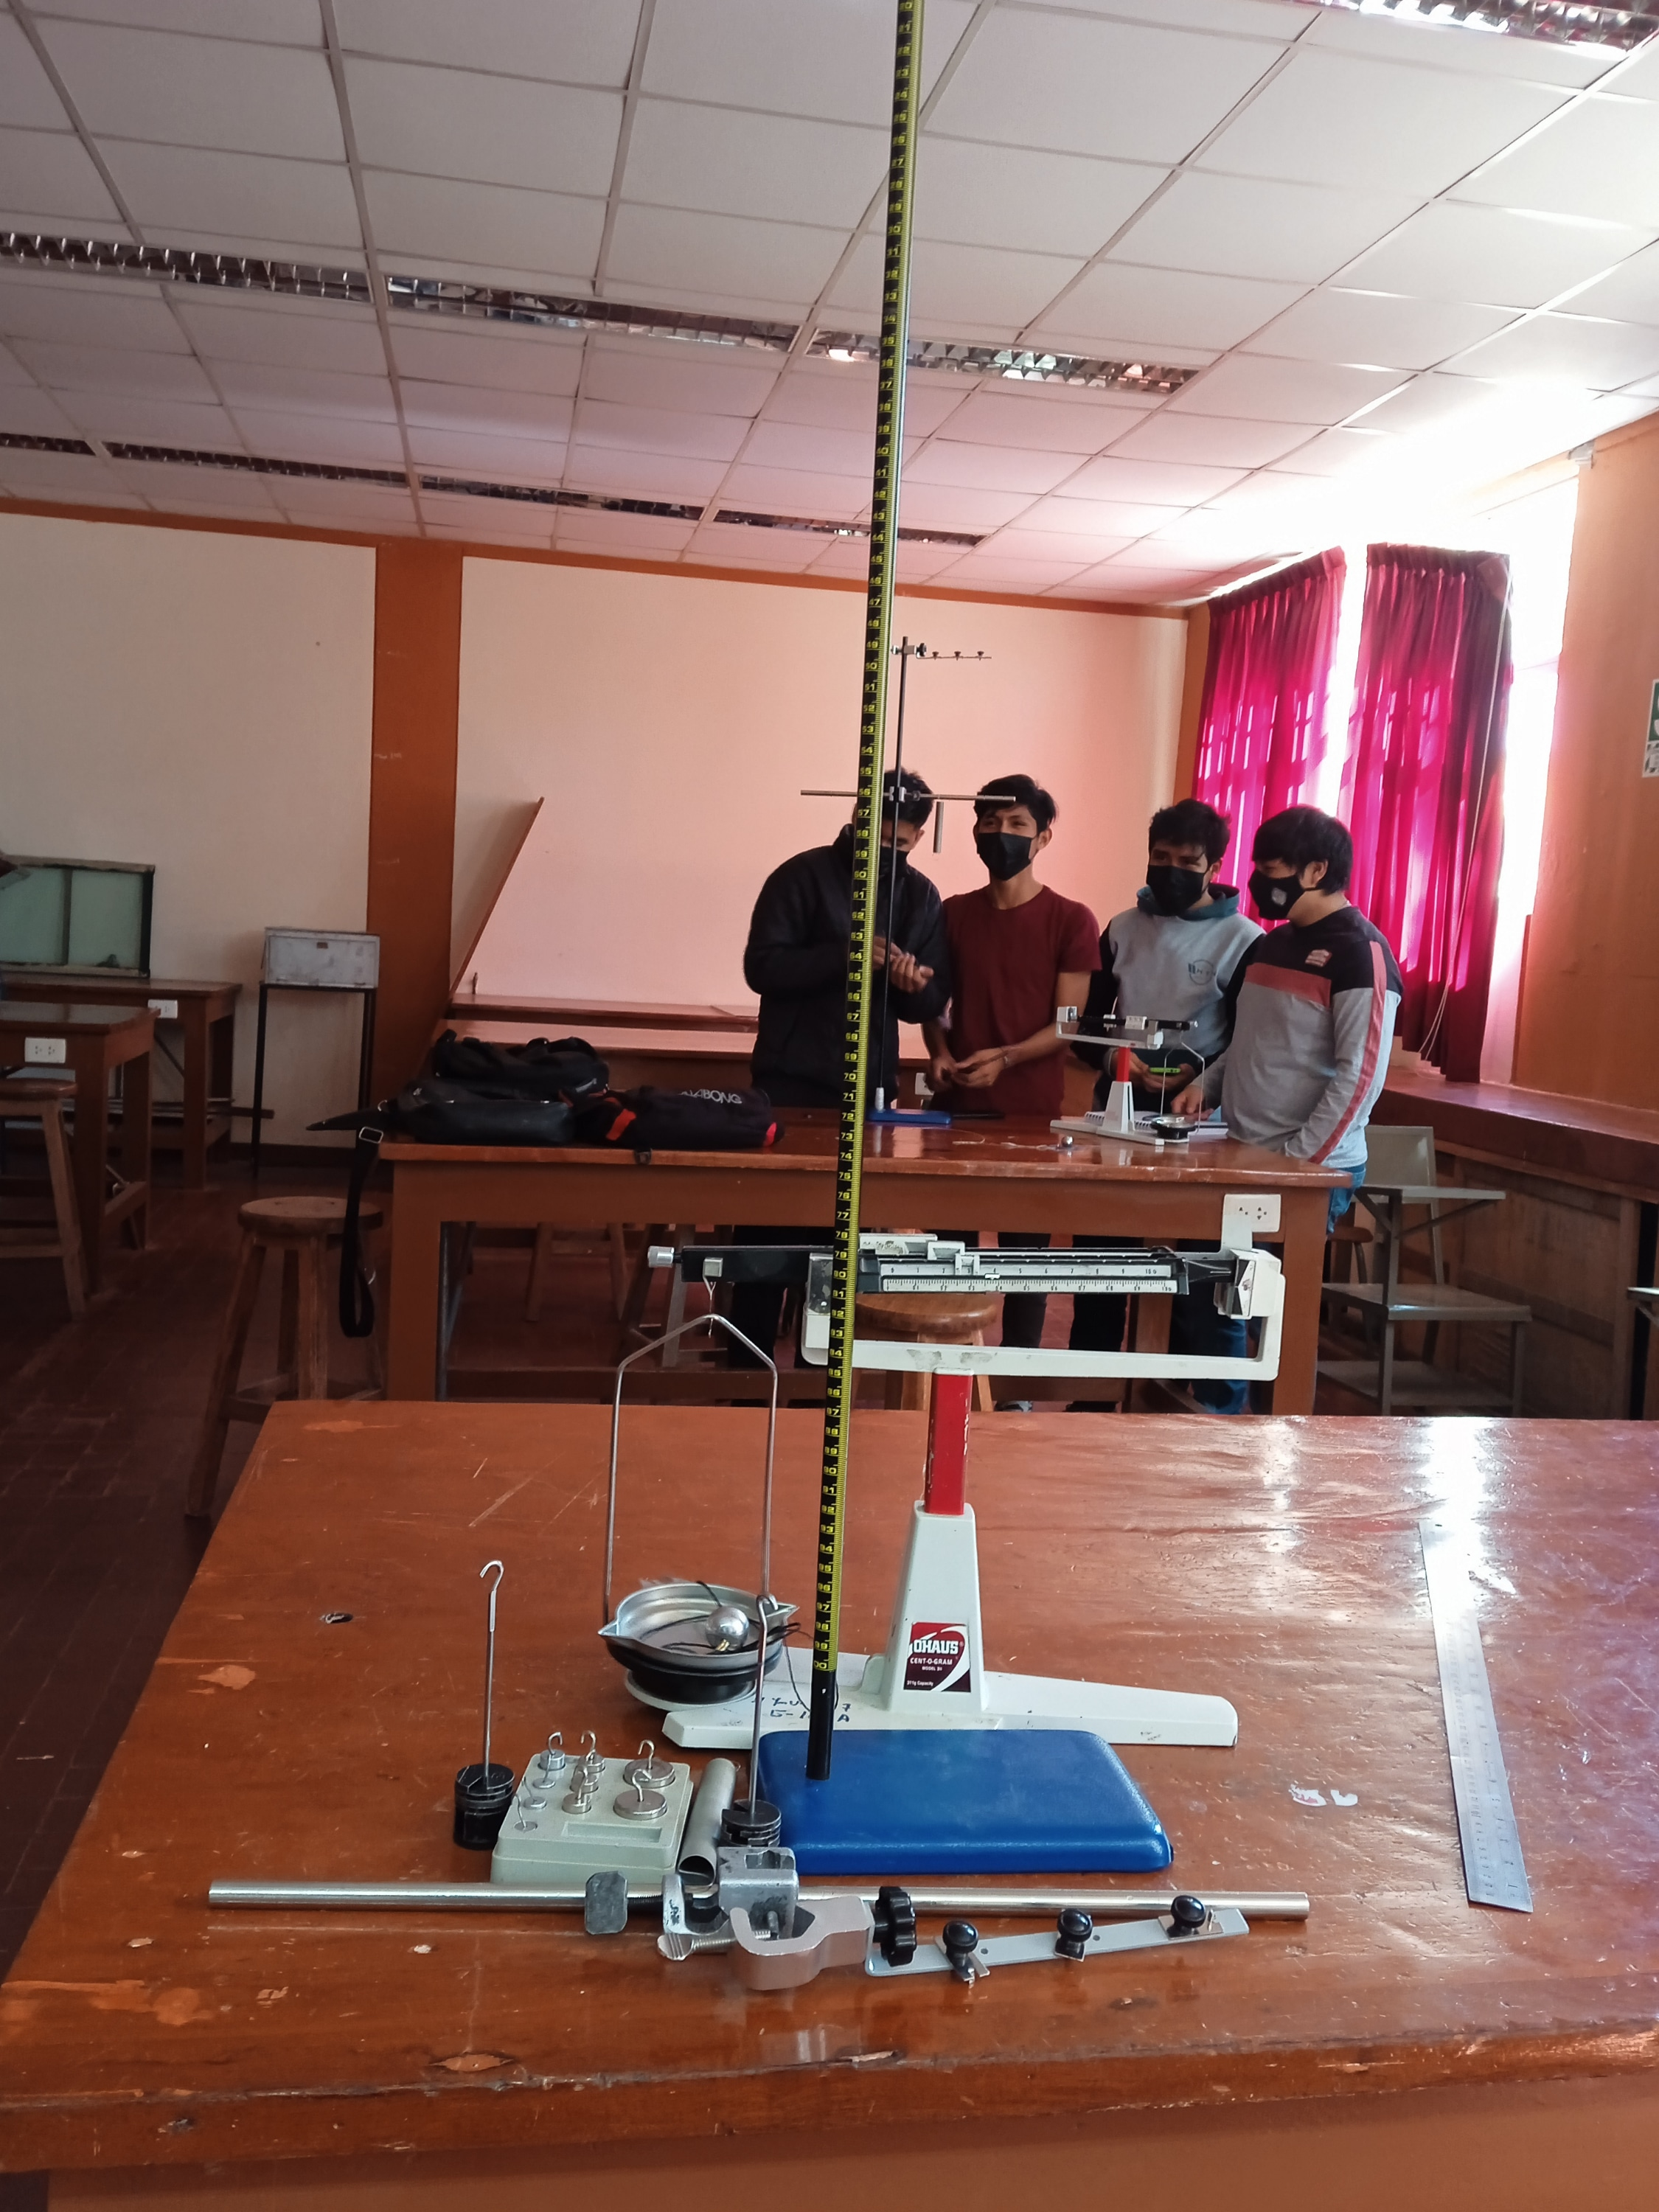
\includegraphics[width=6cm]{Images/materials.jpeg}
		\caption{Materiales utilizados en la práctica de laboratorio.}\label{fig:01}
	\end{figure}

	\begin{figure}[H]
		\centering
		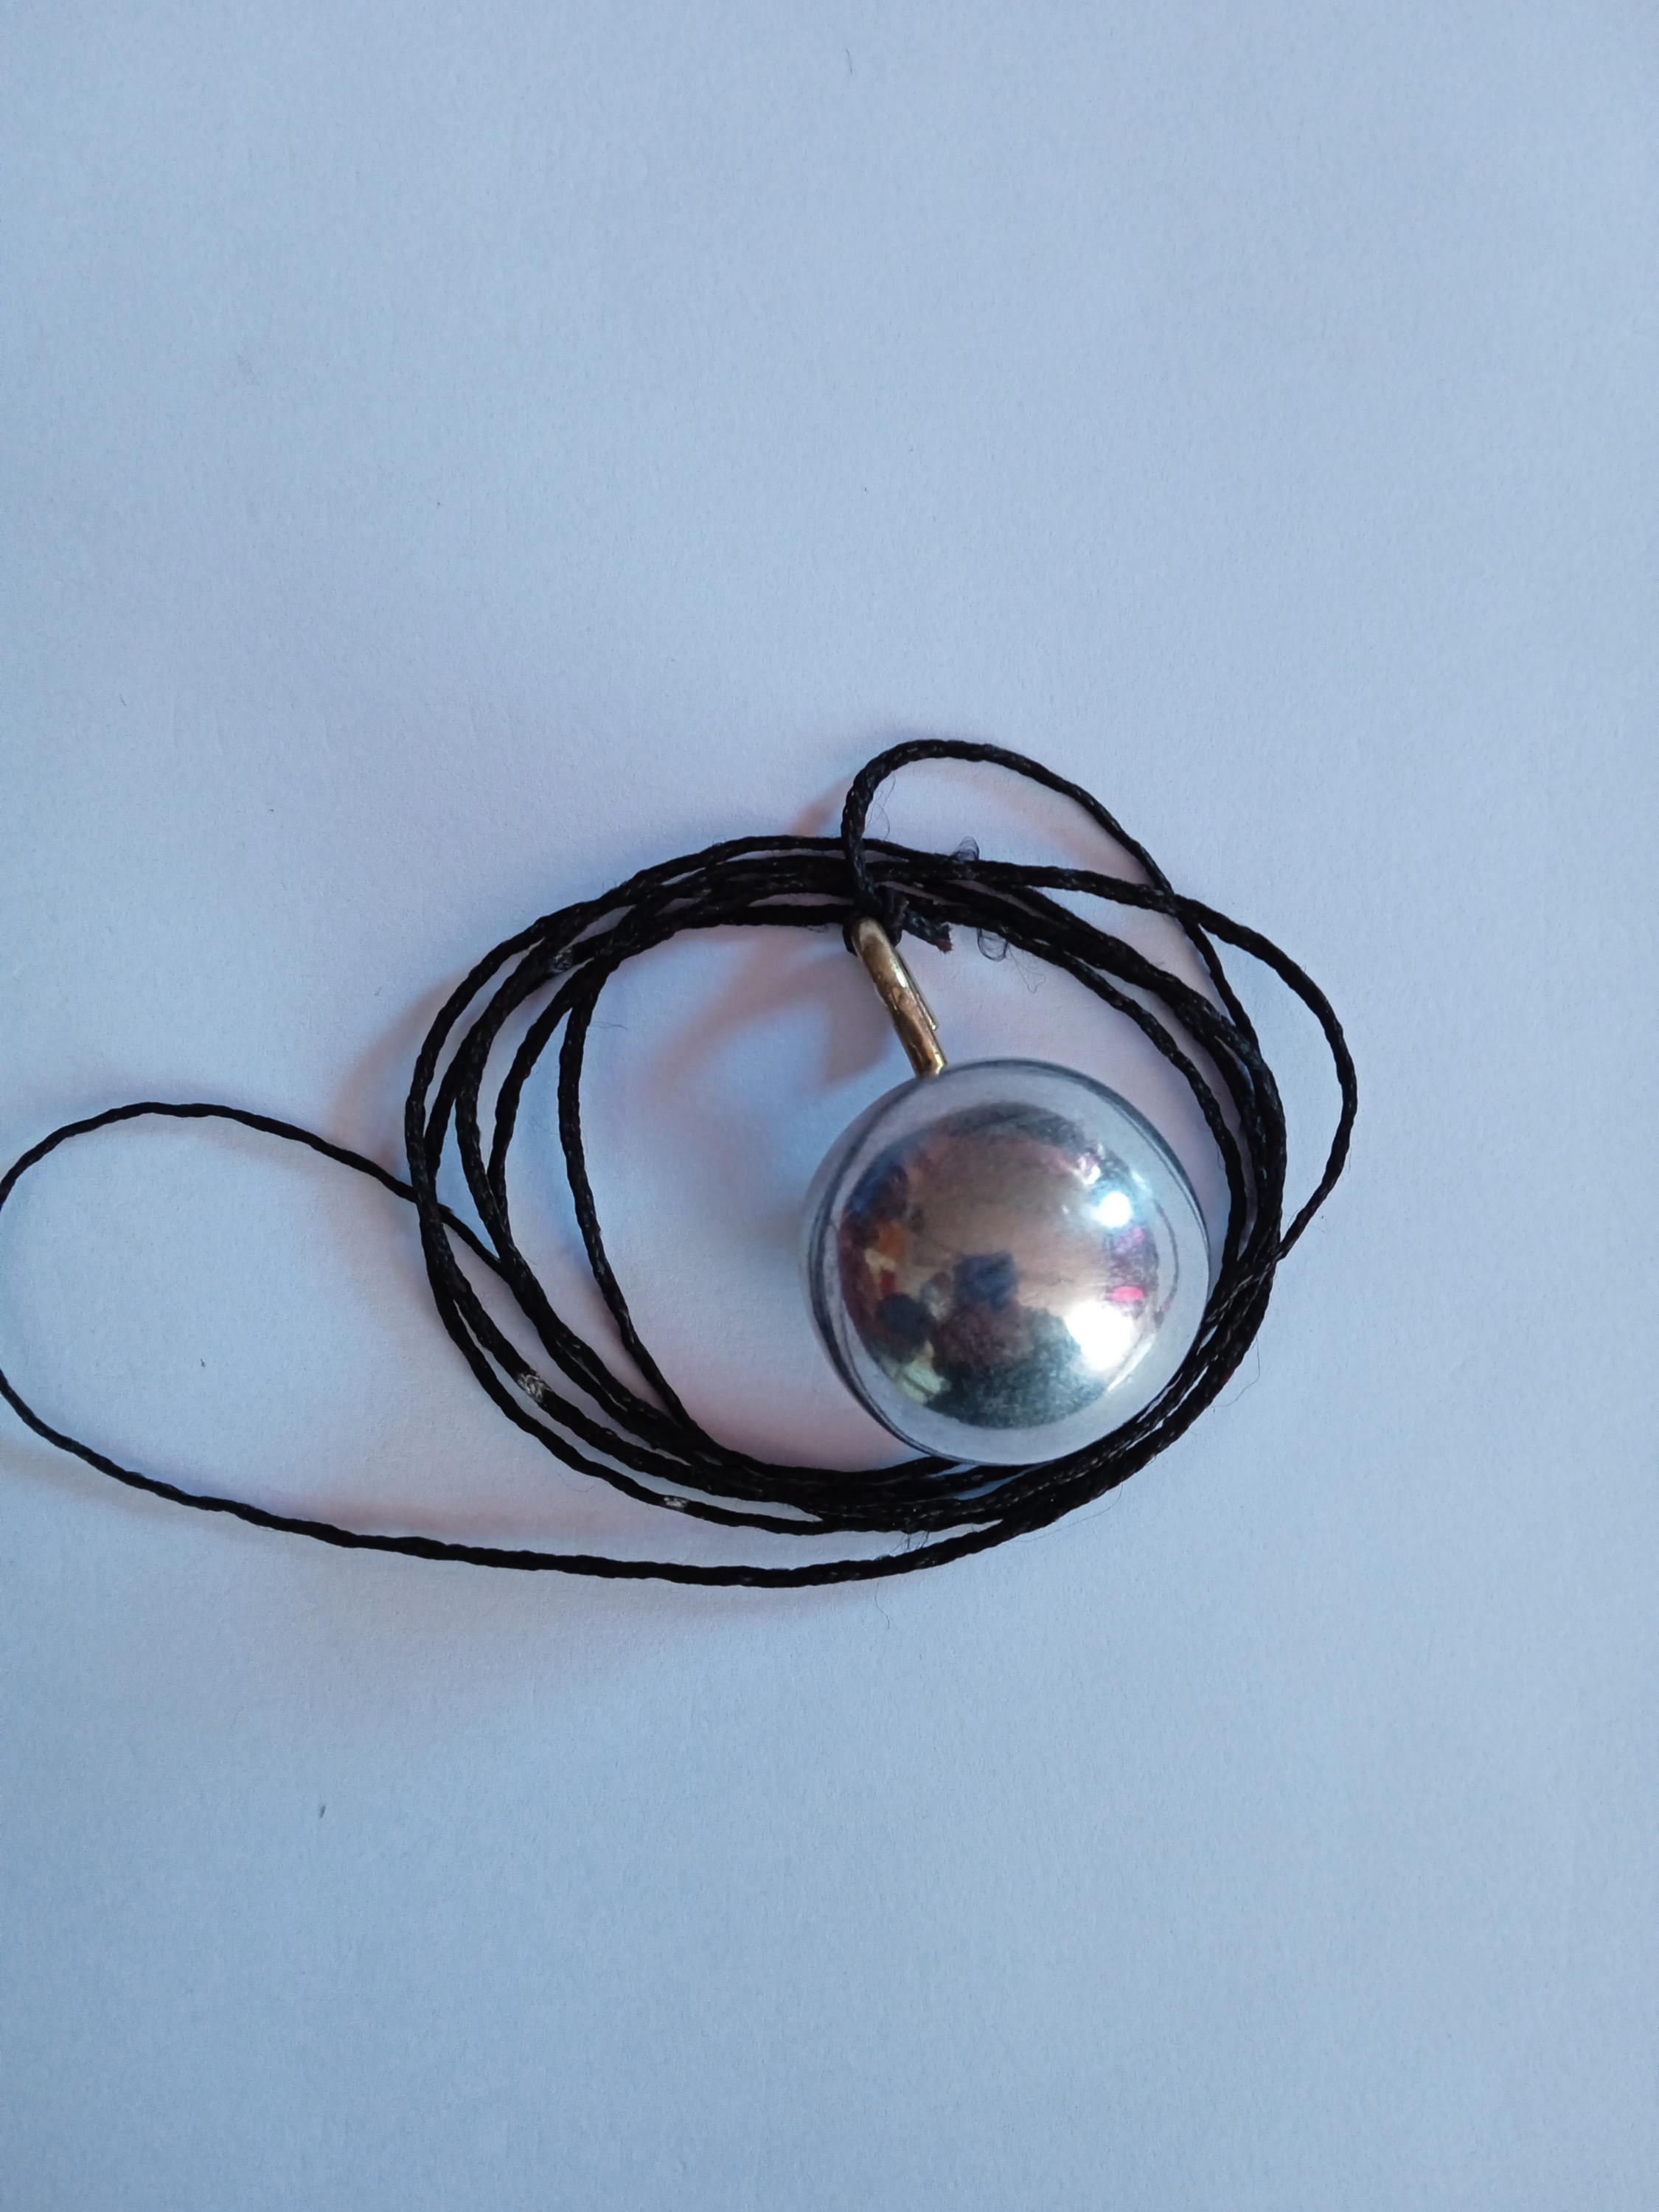
\includegraphics[width=6cm]{Images/masa_hilo.jpeg}
		\caption{Masa (esfera) e hilo.}\label{fig:02}
	\end{figure}
\end{multicols}

%-------------------------------------------------------------------------------------------
\section{Fundamento teórico}
\subsection{Movimiento Armónico Simple (M.A.S)}
\begin{figure}[H]
	\centering
	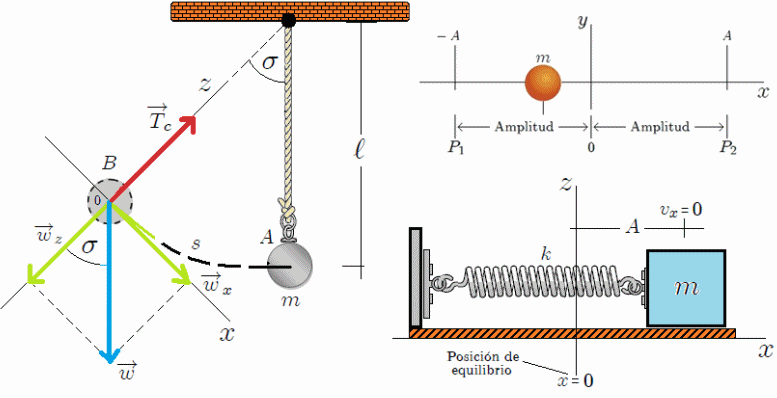
\includegraphics[width=12cm]{Images/fig_02}
	\caption{Movimiento armónico simple.}\label{fig:03}
\end{figure}
El Movimiento Armónico Simple (MAS) es el movimiento periódico más sencillo que se puede analizar, el cual sucede cuando existe una fuerza de restitución $F_R$, la cual es directamente proporcional al desplazamiento x con respecto a un punto equilibrio.
El movimiento armónico simple es la proyección del movimiento circular uniforme sobre un diámetro.
\begin{figure}[H]
	\centering
	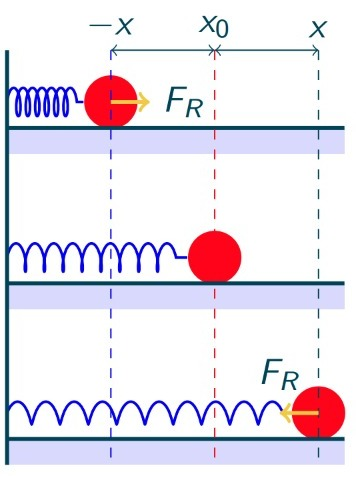
\includegraphics[width=5cm]{Images/fig_i.jpeg}
\end{figure}

\subsubsection{Características del movimiento armónico simple}
\paragraph{Amplitud del movimiento}
\begin{itemize}[label=\textbf{$\bullet$},itemsep=2pt,partopsep=6pt,parsep=6pt]
	\item Se denota con la letra A y se define como la magnitud máxima del desplazamiento con respecto al equilibrio; es decir, el valor máximo de $|x|$ y siempre es positivo.
	\item El rango global del movimiento es 2A.
	\item Las unidades de A depende del fenómeno físico que estemos trabajando.
\end{itemize}
\paragraph{Perido y frecuencia}
\begin{itemize}[label=\textbf{$\bullet$},itemsep=2pt,partopsep=6pt,parsep=6pt]
	\item El periodo se denota con la letra T y se define como el tiempo que tarda en cumplirse un ciclo.
	\item La unidad del periodo en el SI es el segundo, aunque a veces se expresa como segundos por ciclo.
	\item La frecuencia se denota con la letra f, y se define como el número de ciclos por la unidad de tiempo que realiza un movimiento periódico.
	\item La frecuencia se relaciona con el periodo mediante la siguiente relación.
	      \[f=\cfrac{1}{T}\]
	\item La unidad de la frecuencia en el SI es el Hertz ($1hz=$ ciclo/s$=1{s}^{-1}$).
\end{itemize}
\paragraph{Fecuencia angular}
\begin{itemize}[label=\textbf{$\bullet$},itemsep=2pt,partopsep=6pt,parsep=6pt]
	\item La frecuencia angular se denota con la letra $w$, y se define:
	\item La frecuencia representa la rapidezde cambio de una cantidad angular la cual se mide en radianes, de modo que sus unidades son $rad/s$.
\end{itemize}
\subsubsection{Ecuación diferencial del MAS}
\begin{itemize}[label=\textbf{$\bullet$},itemsep=2pt,partopsep=6pt,parsep=6pt]
	\item Si se considera elsistema masa-resorte y se aplica la segunda ley de Newton a la masa m:
	      \[\sum F_x=-kx=ma\]
	\item Usando la definición de la aceleración se tiene:
	      \[-kx=m\cfrac{d^2 x}{dt^2}\]
	\item Finalmente se obtiene la ecuacion diferenacial general del MAS\@.
	      \[\frac{d^2 x}{dt^2}+\omega^2 x=0\]
	      donde la frecuencia angular del sistema se define como
	      \[\omega=\sqrt[]{\cfrac{k}{m}}\]
\end{itemize}
La solución de dicha ecuación diferencial es:
\[x(t)=A\cos (\omega t+ \phi)\]
donde x describe la poisición de la masa y la cosntante $\phi$ es el ángulo de fase, el cual sirve para encontrarlas condiciones iniciales $(x(0)$, $v_x (0)$ y  $a_x(0))$ del movimiento oscilador.
\begin{figure}[H]
	\centering
	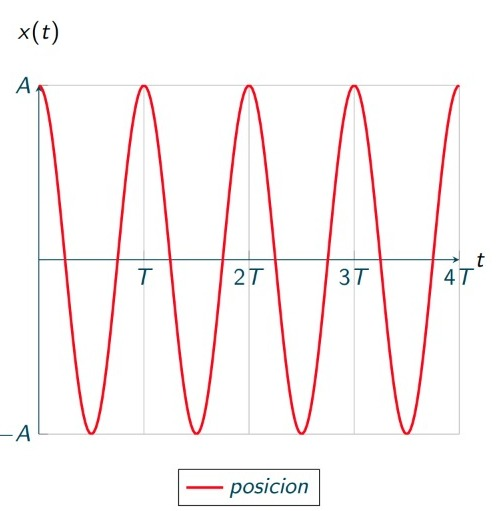
\includegraphics[width=9cm]{Images/min_i.jpeg}
\end{figure}
\subsubsection{Características MAS Sistema masa-resorte}
Para un sistema mas-resorte que describe un MAS las características del movimiento quedan definidas en términos de $\omega$, como por ejemplo.
\begin{itemize}[label=\textbf{$\bullet$},itemsep=2pt,partopsep=6pt,parsep=6pt]
	\item Periodo
	      \[T=\cfrac{2\pi}{\omega}=2\pi \text{ }\sqrt[]{\dfrac{m}{k}}\]
	\item Frecuencia
	      \[f=\cfrac{\omega}{2\pi}=\cfrac{1}{2\pi}\text{ }\sqrt{\cfrac{k}{m}}\]
\end{itemize}
De lo anterior se puede ver que en el MAS descrito por un sistema masa-resorte, el periodo y la frecuencia no dependen de la amplitud.%\ref{fig:04}
\paragraph{Velocidad para un sistema que describe un MAS}
Usando la definición de velocidad se obtiene:
\[v(t)=\cfrac{dx}{dt}=-A\omega \sin (\omega t+\phi)\]
\begin{figure}[H]
	\centering
	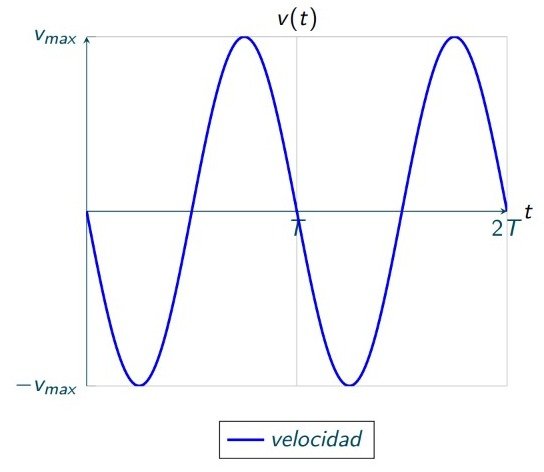
\includegraphics[width=9cm]{Images/min_ii.jpeg}
\end{figure}
\paragraph{Aceleración para una masa que describe un MAS}
Usando la definición de aceleración se obtiene:
\[a(t)=\cfrac{dv}{dt}=-A\omega^2 \cos (\omega t+\phi)\]
\begin{figure}[H]
	\centering
	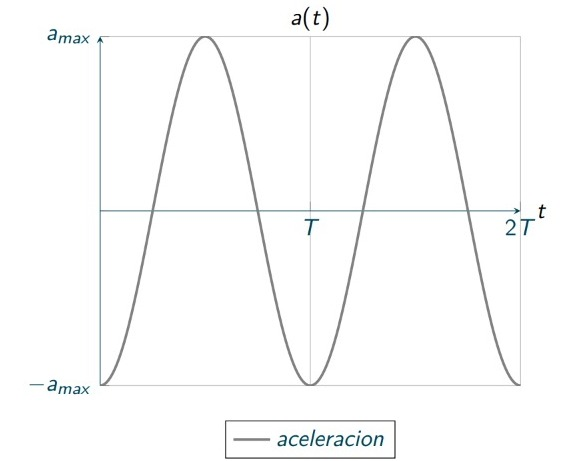
\includegraphics[width=9cm]{Images/min_iii.jpeg}
\end{figure}
%==========================================================================================
\section{Procedimiento y toma de datos}
%-------------------------------------------------------------------------------------------
\subsection{Actividad 1}
\begin{dyNoteImportant}[morado01!20]{azulfor!10}{black!80}{Secuencia de la actividad}
	\begin{enumerate}[label=\itemcirccz{miverde}{\arabic*},itemsep=2pt, leftmargin=0.6cm]
		\item Suspende el resorte y debajo coloque una masa, estire el resorte ligeramente hacia abajo, observe el fenómeno y determine el periodo tomando el tiempo de 10 oscilaciones dos veces.
		\item Discuta con sus compañeros de grupo y calcule la constante k del resorte.
		\item Repita la experiencia para 5 valores de masas diferentes y prepare un cuadro de datos adecuado.
	\end{enumerate}
\end{dyNoteImportant}

\begin{figure}[H]
	\centering
	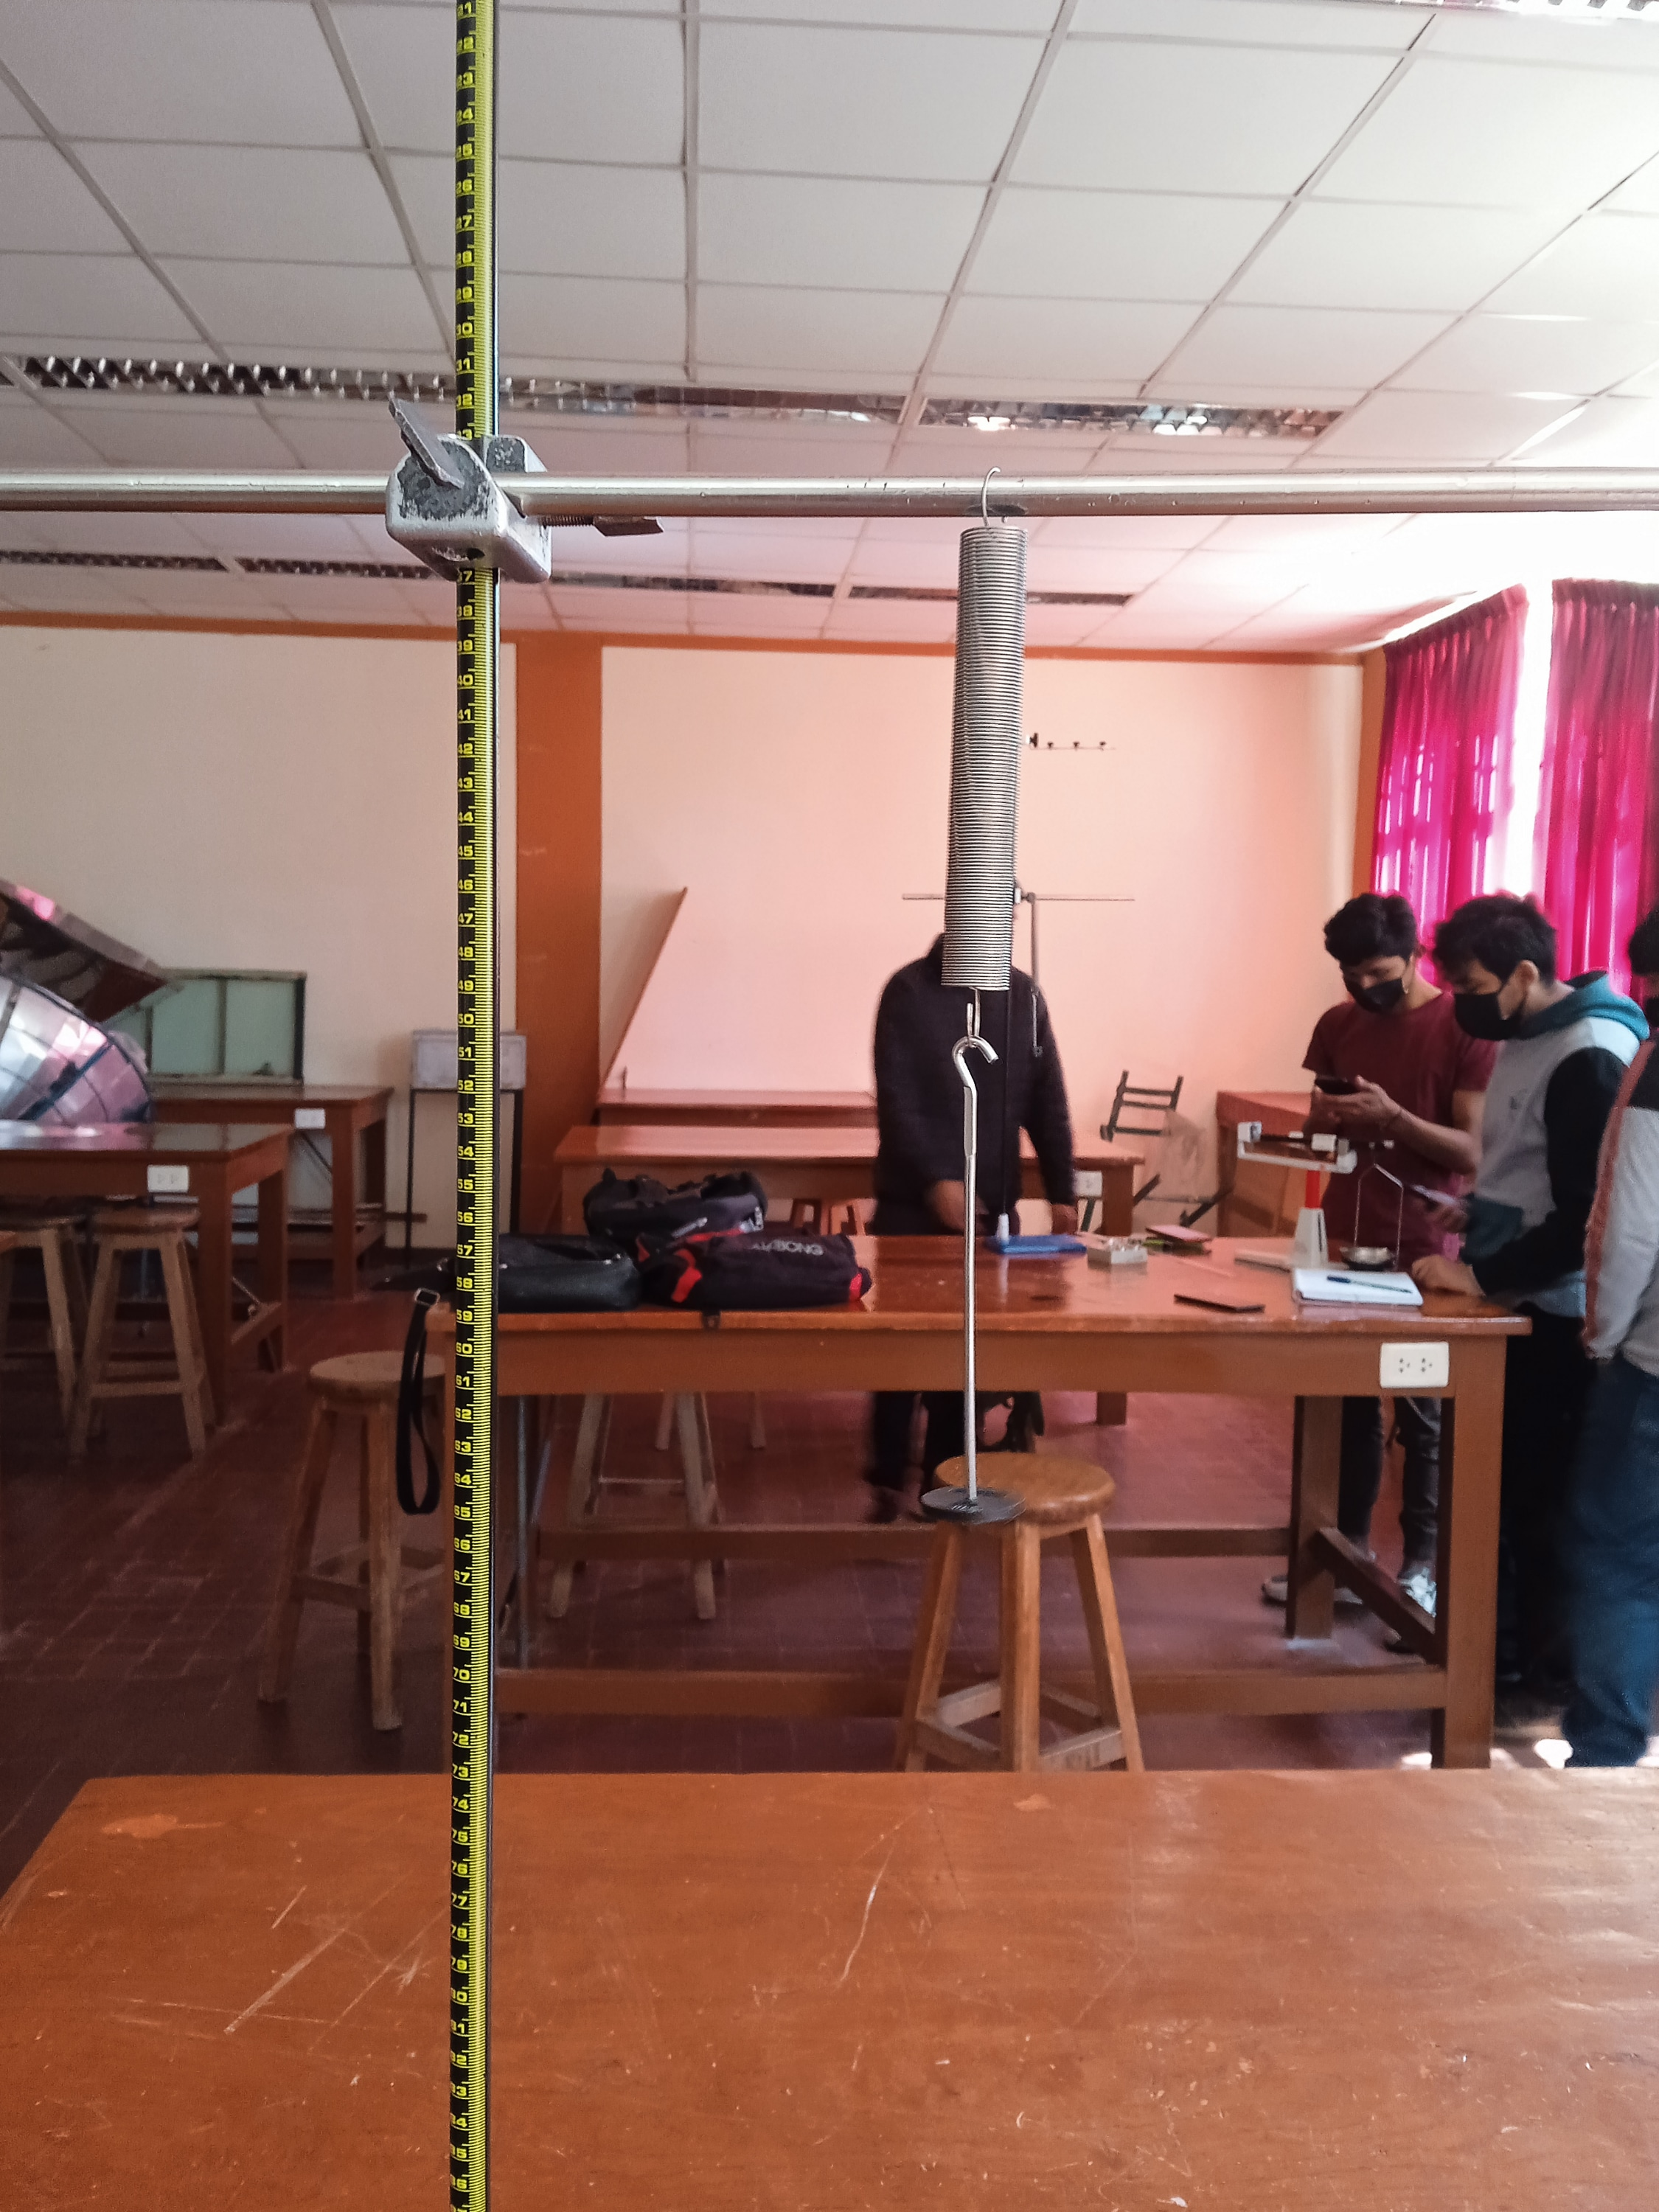
\includegraphics[width=6cm]{Images/spring.jpeg}
	\caption{Experimento MAS masa-resorte.}\label{fig:04}
\end{figure}

\subsubsection{Primer caso}
\begin{enumerate}[label=\bfseries\alph*.-,itemsep=2pt]
	\item \textbf{Calculando el tiempo promedio}
	      \[t_\Delta = \cfrac{t_1+t_2}{2}\]

	      \sdconditions[12cm]{azzul}{Donde:}{%
		      \begin{tabular}{lcl}
			      $t_\Delta$ & \@: & tiempo promedio (en segundos). \\
			      $t_1$      & \@: & tiempo 1 (en segundos).        \\
			      $t_2$      & \@: & tiempo 2 (en segundos).
		      \end{tabular}
	      }

	      \begin{itemize}[label=\textbf{$\bullet$},itemsep=2pt,partopsep=6pt]
		      \item Para el primer evento.
		            \[t_{\Delta{1}}=\cfrac{4.58+4.53}{2}=4.56\]
		      \item Para el segundo evento.
		            \[t_{\Delta{2}}=\cfrac{6.02+6.03}{2}=6.03\]
		      \item Para el tercer evento.
		            \[t_{\Delta{3}}=\cfrac{7.17+7.23}{2}=7.20\]
		      \item Para el cuarto evento.
		            \[t_{\Delta{4}}=\cfrac{8.24+8.18}{2}=8.21\]
		      \item Para el quinto evento.
		            \[t_{\Delta{5}}=\cfrac{9.09+9.13}{2}=9.11\]
	      \end{itemize}
	\item \textbf{Calculando el periodo}
	      \[T = \dfrac{t_\Delta}{10}\]
	      \begin{itemize}[label=\textbf{$\bullet$},itemsep=2pt,partopsep=6pt]
		      \item Para el primer evento.
		            \[T_1 = \dfrac{4.56}{10}=0.46\]
		      \item Para el segundo evento.
		            \[T_2 = \dfrac{6.03}{10}=0.60\]
		      \item Para el tercer evento.
		            \[T_3 = \dfrac{7.20}{10}=0.72\]
		      \item Para el cuarto evento.
		            \[T_4 = \dfrac{8.21}{10}=0.82\]
		      \item Para el quinto evento.
		            \[T_5 = \dfrac{9.11}{10}=0.91\]
	      \end{itemize}

	\item \textbf{Calculando la constante de rigidez}
	      \[k= \cfrac{4\pi^2 m}{T^2}\]

	      \sdconditions[12cm]{azzul}{Donde:}{%
		      \begin{tabular}{lcl}
			      $k$ & \@: & constante de rigidez.  \\
			      $m$ & \@: & masa (en Kilogramos).  \\
			      $T$ & \@: & periodo (en segundos).
		      \end{tabular}
	      }

	      \begin{itemize}[label=\textbf{$\bullet$},itemsep=2pt,partopsep=6pt]
		      \item Para el primer evento.
		            \[k_1= \cfrac{4\times\pi^2\times{0.04}}{{0.46}^2}=7.61\]
		      \item Para el segundo evento.
		            \[k_2= \cfrac{4\times\pi^2\times{0.07}}{{0.6}^2}=7.61\]
		      \item Para el tercer evento.
		            \[k_3= \cfrac{4\times\pi^2\times{0.1}}{{0.72}^2}=7.62\]
		      \item Para el cuarto evento.
		            \[k_4= \cfrac{4\times\pi^2\times{0.13}}{{0.82}^2}=7.61\]
		      \item Para el quinto evento.
		            \[k_5= \cfrac{4\times\pi^2\times{0.16}}{{0.91}^2}=7.61\]
	      \end{itemize}
\end{enumerate}

\subsubsection{Segundo caso}
\begin{enumerate}[label=\bfseries\alph*.-,itemsep=2pt]
	\item \textbf{Calculando la variación de x}
	      \[\Delta x= \cfrac{x_f-x_i}{2}\]
	      \begin{itemize}[label=\textbf{$\bullet$},itemsep=2pt,partopsep=6pt,parsep=6pt]
		      \item Para el primer evento.
		            \[\Delta x_1= \cfrac{15.75-10.6}{2}=2.58cm<>0.3m\]
		      \item Para el segundo evento.
		            \[\Delta x_2= \cfrac{19.6-10.6}{2}=4.5cm<>0.05m\]
		      \item Para el tercer evento.
		            \[\Delta x_3= \cfrac{23.46-10.6}{2}=6.43cm<>0.06m\]
		      \item Para el cuarto evento.
		            \[\Delta x_4= \cfrac{27.33-10.6}{2}=8.37cm<>0.08m\]
		      \item Para el quinto evento.
		            \[\Delta x_5= \cfrac{31.2-10.6}{2}=10.3cm<>0.10m\]
	      \end{itemize}

	\item \textbf{Calculando la constante de rigidez}
	      \[k= \cfrac{F}{x}\]

	      \sdconditions[12cm]{azzul}{Donde:}{%
		      \begin{tabular}{lcl}
			      $k$ & \@: & constante de rigidez.    \\
			      $F$ & \@: & fuerza (en newtons).     \\
			      $x$ & \@: & deformación (en metros).
		      \end{tabular}
	      }
	      \begin{itemize}[label=\textbf{$\bullet$},itemsep=2pt,partopsep=6pt,parsep=6pt]
		      \item Para el primer evento.
		            \[k_1= \cfrac{0.04\times{9.8}}{x}=7.61\]
		      \item Para el segundo evento.
		            \[k_2= \cfrac{0.07\times{9.8}}{x}=7.62\]
		      \item Para el tercer evento.
		            \[k_3= \cfrac{0.1\times{9.8}}{x}=7.62\]
		      \item Para el cuarto evento.
		            \[k_4= \cfrac{0.13\times{9.8}}{x}=7.62\]
		      \item Para el quinto evento.
		            \[k_5= \cfrac{0.16\times{9.8}}{x}=7.61\]
	      \end{itemize}
\end{enumerate}

%-------------------------------------------------------------------------------------------
\subsection{Actividad 2}
\begin{dyNoteImportant}[morado01!20]{azulfor!10}{black!80}{Secuencia de la actividad}
	\begin{enumerate}[label=\itemcirccz{miverde}{\arabic*},itemsep=2pt, leftmargin=0.6cm]
		\item Mida la longitud del péndulo y el periodo del péndulo tomando el tiempo de 10 oscilaciones dos veces, repita esta experiencia para 5 masas diferentes y anote en la tabla.
		\item Varíe la longitud del péndulo 5 veces y determine el periodo tomando el tiempo de 10 oscilaciones.
		\item Grafique $T^2$ en función a $L$ y calcule a partir de ella $g$.
		\item Tome el péndulo de una longitud determinada, variando cinco veces la masa, mide dos veces en cada caso, el tiempo que tarda 10 oscilaciones.
	\end{enumerate}
\end{dyNoteImportant}

\begin{figure}[H]
	\centering
	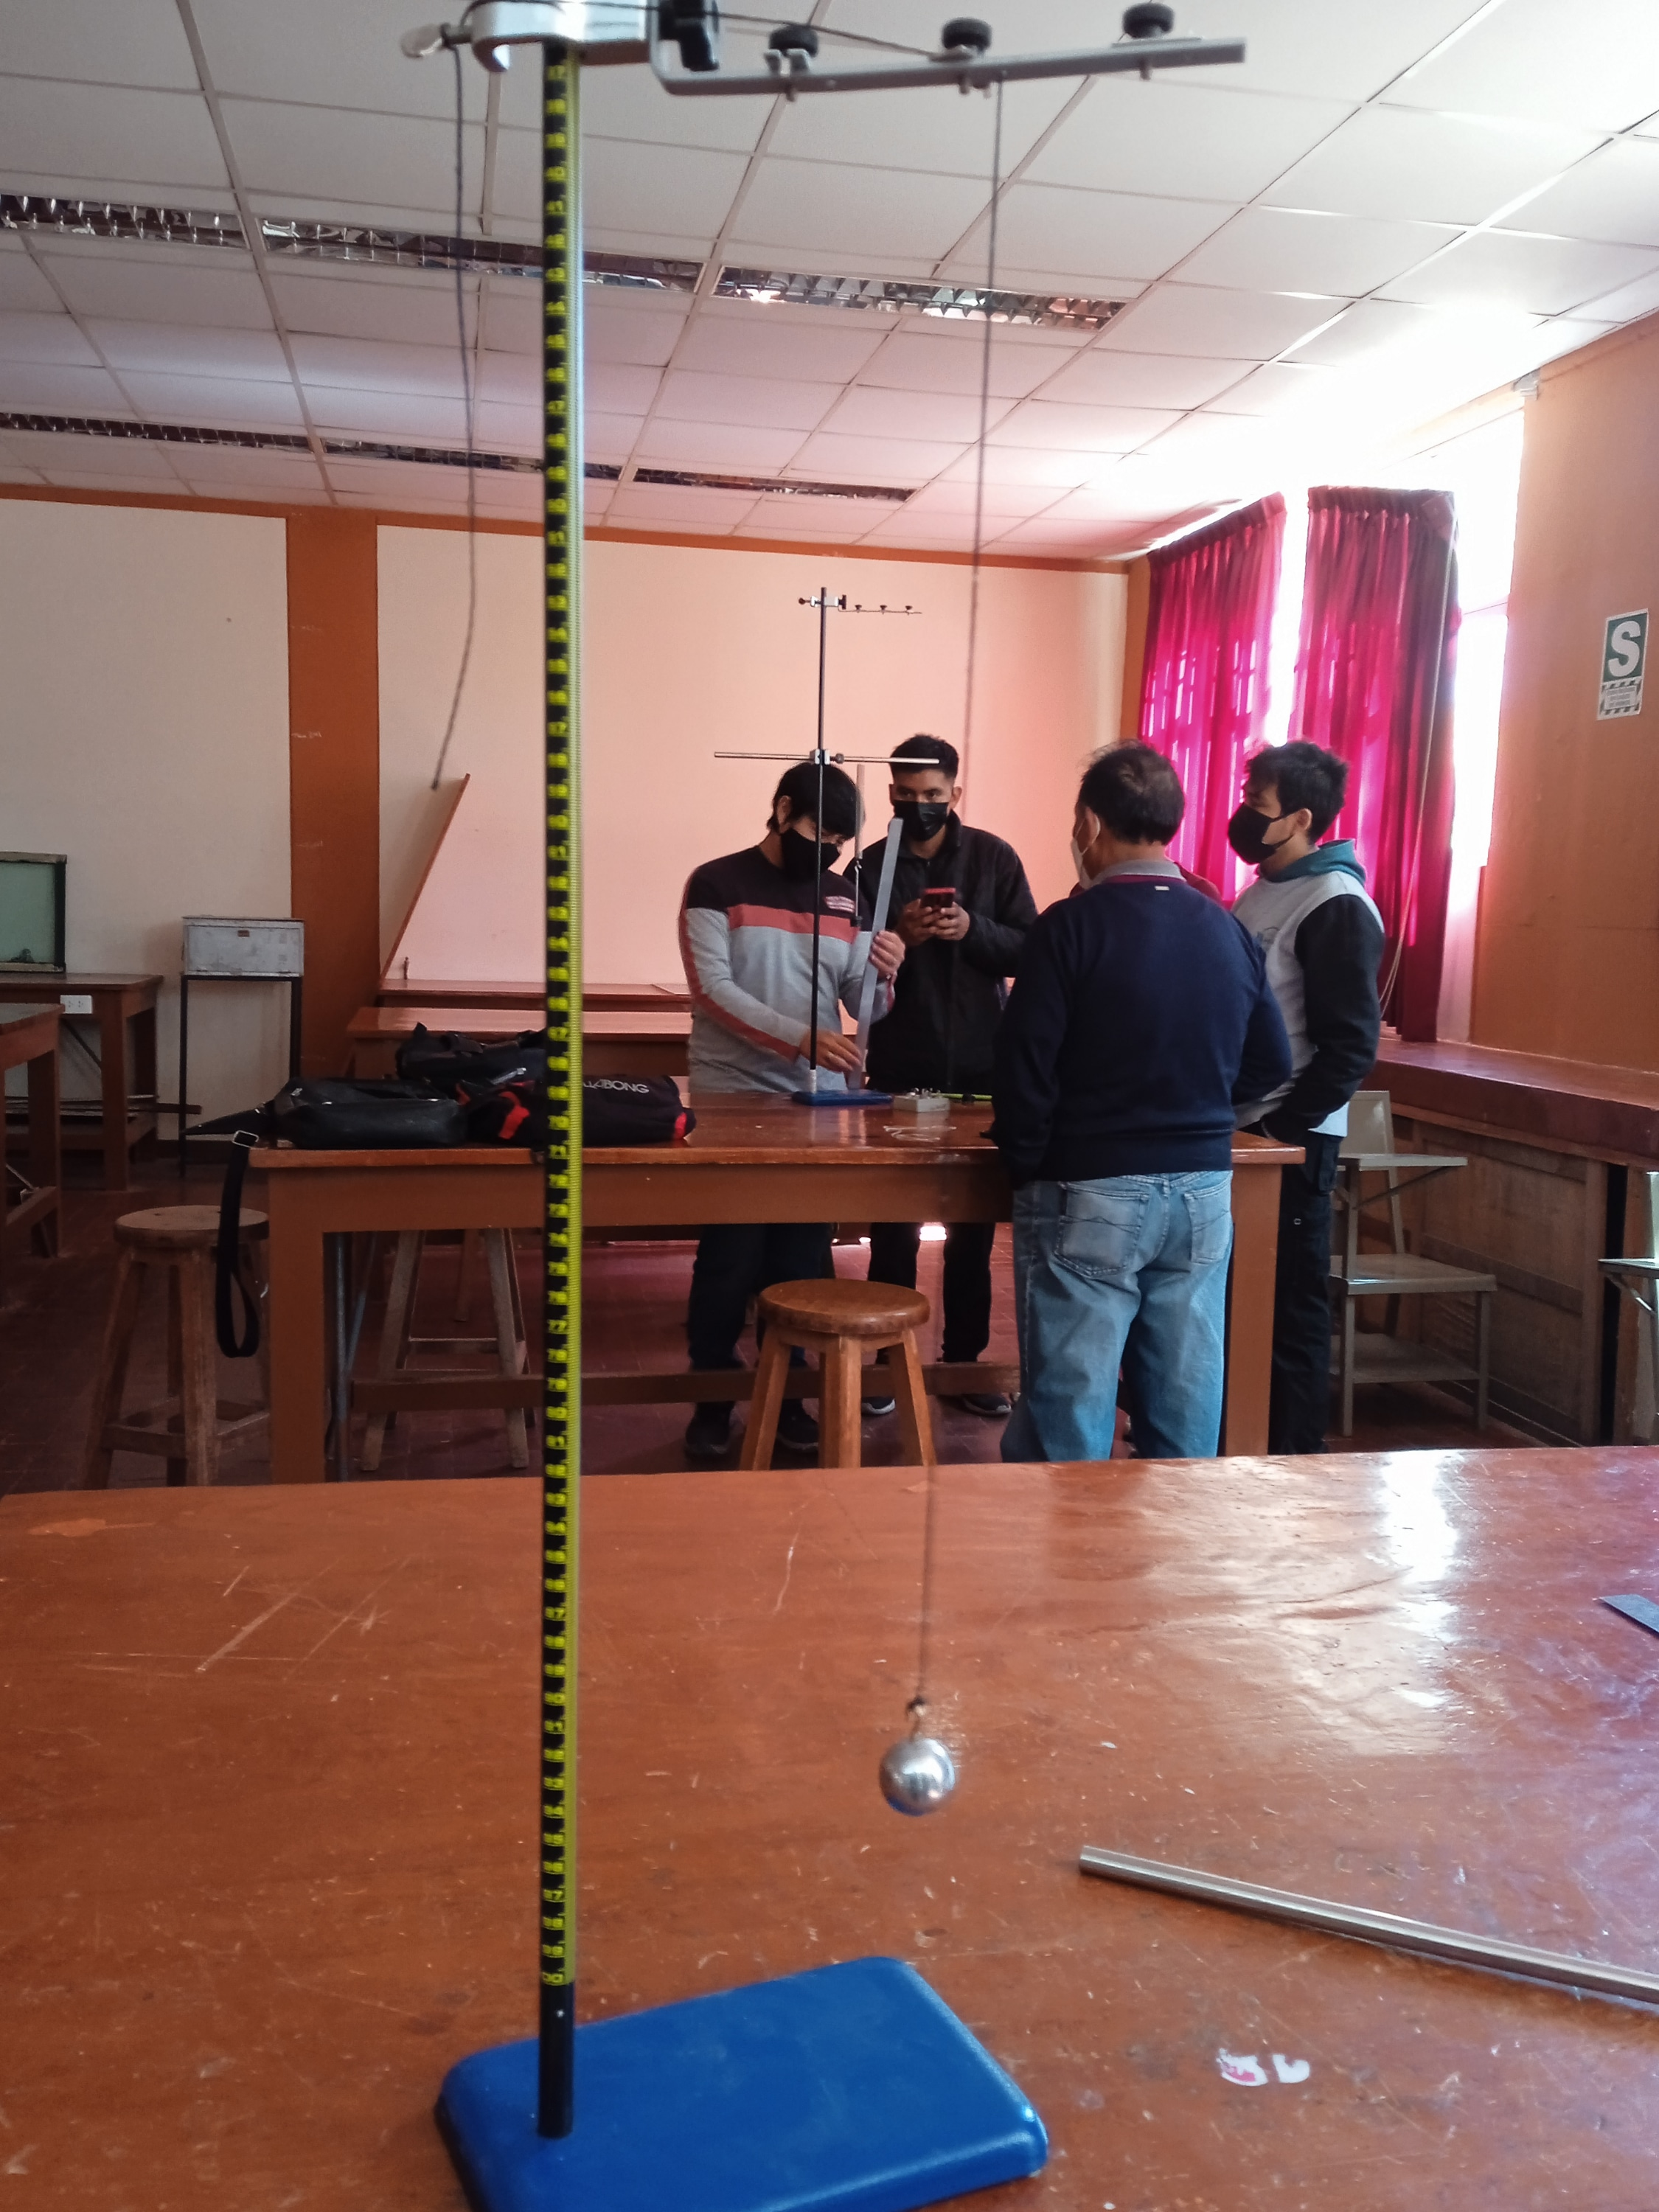
\includegraphics[width=6cm]{Images/pendulum.jpeg}
	\caption{Experimento MAS pendulo simple.}\label{fig:05}
\end{figure}

\subsubsection{Para la longitud constante}
\begin{enumerate}[label=\bfseries\alph*.-,itemsep=2pt]
	\item \textbf{Calculando el tiempo promedio}
	      \[t_\Delta = \cfrac{t_1+t_2}{2}\]
	      \begin{itemize}[label=\textbf{$\bullet$},itemsep=2pt,partopsep=6pt,parsep=6pt]
		      \item Para el primer  evento.
		            \[t_{\Delta{1}}=\cfrac{17.45+17.40}{2}=17.43\]
		      \item Para el segundo evento.
		            \[t_{\Delta{2}}=\cfrac{17.41+17.38}{2}=17.4\]
		      \item Para el tercer  evento.
		            \[t_{\Delta{3}}=\cfrac{17.45+17.55}{2}=17.5\]
		      \item Para el cuarto  evento.
		            \[t_{\Delta{4}}=\cfrac{17.42+17.53}{2}=17.48\]
		      \item Para el quinto  evento.
		            \[t_{\Delta{5}}=\cfrac{17.42+17.50}{2}=17.46\]
	      \end{itemize}

	\item \textbf{Calculando el periodo}
	      \[T = \dfrac{t_\Delta}{10}\]
	      \begin{itemize}[label=\textbf{$\bullet$},itemsep=2pt,partopsep=6pt,parsep=6pt]
		      \item Para el primer evento.
		            \[T_1 = \dfrac{17.43}{10}=1.74\]
		      \item Para el segundo evento.
		            \[T_2 = \dfrac{17.4}{10}=1.74\]
		      \item Para el tercer evento.
		            \[T_3 = \dfrac{17.5}{10}=1.75\]
		      \item Para el cuarto evento.
		            \[T_4 = \dfrac{17.48}{10}=1.75\]
		      \item Para el quinto evento.
		            \[T_5 = \dfrac{17.46}{10}=1.75\]
	      \end{itemize}

	\item \textbf{Calculando la aceleración de la gravedad}
	      \[g= \cfrac{4\pi^2L}{T^2}\]
	      \begin{itemize}[label=\textbf{$\bullet$},itemsep=2pt,partopsep=6pt,parsep=6pt]
		      \item Para el primer evento.
		            \[g_1= \cfrac{4\times\pi^2\times{0.75}}{{1.74}^2}=9.77\]
		      \item Para el segundo evento.
		            \[g_2= \cfrac{4\times\pi^2\times{0.75}}{{1.74}^2}=9.77\]
		      \item Para el tercer evento.
		            \[g_3= \cfrac{4\times\pi^2\times{0.75}}{{1.75}^2}=9.66\]
		      \item Para el cuarto evento.
		            \[g_4= \cfrac{4\times\pi^2\times{0.75}}{{1.75}^2}=9.66\]
		      \item Para el quinto evento.
		            \[g_5= \cfrac{4\times\pi^2\times{0.75}}{{1.75}^2}=9.66\]
	      \end{itemize}
\end{enumerate}

\subsubsection{Para la masa constante}
\begin{enumerate}[label=\bfseries\alph*.-,itemsep=2pt]
	\item \textbf{Calculando el tiempo promedio}
	      \[t_\Delta = \cfrac{t_1+t_2}{2}\]
	      \begin{itemize}[label=\textbf{$\bullet$},itemsep=2pt,partopsep=6pt,parsep=6pt]
		      \item Para el primer  evento.
		            \[t_{\Delta{1}}=\cfrac{17.43+17.58}{2}=17.51\]
		      \item Para el segundo evento.
		            \[t_{\Delta{2}}=\cfrac{15.51+15.60}{2}=15.56\]
		      \item Para el tercer  evento.
		            \[t_{\Delta{3}}=\cfrac{13.55+13.47}{2}=13.51\]
		      \item Para el cuarto  evento.
		            \[t_{\Delta{4}}=\cfrac{11.15+11.06}{2}=11.11\]
		      \item Para el quinto  evento.
		            \[t_{\Delta{5}}=\cfrac{7.95+7.64}{2}=7.8\]
	      \end{itemize}

	\item \textbf{Calculando el periodo}
	      \[T = \dfrac{t_\Delta}{10}\]
	      \begin{itemize}[label=\textbf{$\bullet$},itemsep=2pt,partopsep=6pt,parsep=6pt]
		      \item Para el primer evento.
		            \[T_1 = \dfrac{17.51}{10}=1.75\]
		      \item Para el segundo evento.
		            \[T_2 = \dfrac{15.56}{10}=1.56\]
		      \item Para el tercer evento.
		            \[T_3 = \dfrac{13.51}{10}=1.35\]
		      \item Para el cuarto evento.
		            \[T_4 = \dfrac{11.11}{10}=1.11\]
		      \item Para el quinto evento.
		            \[T_5 = \dfrac{7.8}{10}=0.78\]
	      \end{itemize}

	\item \textbf{Calculando la aceleración de la gravedad}
	      \[g= \cfrac{4\pi^2L}{T^2}\]
	      \begin{itemize}[label=\textbf{$\bullet$},itemsep=2pt,partopsep=6pt,parsep=6pt]
		      \item Para el primer evento.
		            \[g_1= \cfrac{4\times\pi^2\times{0.75}}{{1.75}^2}=9.7\]
		      \item Para el segundo evento.
		            \[g_2= \cfrac{4\times\pi^2\times{0.60}}{{1.56}^2}=9.7\]
		      \item Para el tercer evento.
		            \[g_3= \cfrac{4\times\pi^2\times{0.45}}{{1.35}^2}=9.7\]
		      \item Para el cuarto evento.
		            \[g_4= \cfrac{4\times\pi^2\times{0.30}}{{1.11}^2}=9.6\]
		      \item Para el quinto evento.
		            \[g_5= \cfrac{4\times\pi^2\times{0.15}}{{0.78}^2}=9.7\]
	      \end{itemize}
\end{enumerate}

%==========================================================================================
\section{Tabla y resultados}
\begin{table}[H]
	\centering
	\parbox{10cm}{%
		\caption{Cálculo de la constante de rigidez ($k$).}\label{tab:03}}\\
	\sdconditions[12cm]{azzul}{Para:}{%
		\begin{tabular}{lcl}
			$m$   & \@: & Masa (en kg).                       \\
			$t_1$, $t_2$ y $t_\Delta$ & \@: & Tiempo (en segundos). \\
			$T$ & \@: & Periodo (en segundos). \\
			$K$   & \@: & Constante ed rigidez (en $N/m$).
		\end{tabular}
	}
	\begin{tabular}{C{0.5cm}C{1cm}C{1cm}C{1cm}C{1cm}C{1cm}C{1cm}}
		\hline
		\rowcolor{gray!10}$N$ & $m$    & $t_1$  & $t_2$  & $t_\Delta$ & $T$    & $K$    \\
		\hline
		1                     & $0.4$  & $4.58$ & $4.53$ & $4.56$     & $0.46$ & $7.61$ \\
		2                     & $0.7$  & $6.02$ & $6.03$ & $6.03$     & $0.60$ & $7.61$ \\
		3                     & $0.1$  & $7.17$ & $7.23$ & $7.20$     & $0.72$ & $7.62$ \\
		4                     & $0.13$ & $8.24$ & $8.18$ & $8.21$     & $0.82$ & $7.61$ \\
		5                     & $0.16$ & $9.09$ & $9.13$ & $9.11$     & $0.91$ & $7.61$ \\
		\midrule
	\end{tabular}
\end{table}
\begin{table}[H]
	\centering
	\parbox{7cm}{%
		\caption{Cálculo de la constante de rigidez ($k$).}\label{tab:04}}\\
	\sdconditions[12cm]{azzul}{Para:}{%
		\begin{tabular}{lcl}
			$F$   & \@: & Fuerza (en Newtons)                       \\
			$x_i$ & \@: & Resorte sin deformación (en centímetros). \\
			$x_f$ & \@: & Resorte con deformación (en centímetros). \\
			$x_m$ & \@: & Deformación (en metros).                  \\
			$K$   & \@: & Constante ed rigidez (en $N/m$).
		\end{tabular}
	}
	\begin{tabular}{C{0.5cm}C{1cm}C{1cm}C{1cm}C{1cm}C{1cm}}
		\hline
		\rowcolor{gray!10}$N$ & $F$    & $x_i$  & $x_f$   & $x_m$  & $K$    \\ \hline
		1                     & $0.04$ & $10.6$ & $15.75$ & $0.04$ & $7.61$ \\
		2                     & $0.07$ & $10.6$ & $19.6$  & $0.05$ & $7.62$ \\
		3                     & $0.1$  & $10.6$ & $23.46$ & $0.06$ & $7.62$ \\
		4                     & $0.13$ & $10.6$ & $27.33$ & $0.08$ & $7.62$ \\
		5                     & $0.16$ & $10.6$ & $31.2$  & $0.10$ & $7.61$ \\
		\midrule
	\end{tabular}
\end{table}
%====================================================$
\begin{table}[H]
	\centering
	\parbox{9cm}{%
		\caption{Cálculo de la gravedad.}\label{tab:01}}\\
	\sdconditions[12cm]{azzul}{Para:}{%
		\begin{tabular}{lcl}
			$m_1$                   & \@: & $23.35$gr. $<>0.03$kg. \\
			$t_1, t_2$ y $t_\Delta$ & \@: & tiempo (en seundos).   \\
			$T$                     & \@: & Periodo (en Hertz).    \\
			$g$                     & \@: & gravedad (en $m/s^2$).
		\end{tabular}
	}
	\begin{tabular}{C{0.35cm}C{1.3cm}C{1cm}C{1cm}C{1cm}C{1cm}C{1cm}}
		\hline
		\rowcolor{gray!10} $N$ & $m$      & $t_1$   & $t_2$   & $t_\Delta $ & $T$    & $g$    \\
		\hline
		1                      & $m_1$    & $17.45$ & $17.40$ & $17.43$     & $1.74$ & $9.77$ \\
		2                      & $m_1+2$  & $17.41$ & $17.38$ & $17.4$      & $1.74$ & $9.77$ \\
		3                      & $m_1+5$  & $17.45$ & $17.55$ & $17.5$      & $1.75$ & $9.66$ \\
		4                      & $m_1+10$ & $17.42$ & $17.53$ & $17.48$     & $1.75$ & $9.66$ \\
		5                      & $m_1+20$ & $17.42$ & $17.50$ & $17.46$     & $1.75$ & $9.66$ \\
		\midrule
	\end{tabular}
\end{table}

\begin{table}[H]
	\centering
	\parbox{10cm}{%
		\caption{Cálculo de la gravedad.}\label{tab:02}}\\
	\sdconditions[12cm]{azzul}{Para:}{%
		\begin{tabular}{lcl}
			$L$                     & \@: & Longitud (en metros)   \\
			$t_1, t_2$ y $t_\Delta$ & \@: & tiempo (en seundos).   \\
			$T$                     & \@: & Periodo (en segundos).    \\
			$g$                     & \@: & gravedad (en $m/s^2$).
		\end{tabular}
	}
	\begin{tabular}{C{0.5cm}C{1cm}C{1cm}C{1cm}C{1cm}C{1cm}C{1cm}}
		\hline
		\rowcolor{gray!10} $N$ & $L$  & $t_1$   & $t_2$   & $t_\Delta$ & $T$    & $g$   \\
		\hline
		1                      & $75$ & $17.43$ & $17.58$ & $17.51$    & $1.75$ & $9.7$ \\
		2                      & $60$ & $15.51$ & $15.60$ & $15.56$    & $1.56$ & $9.7$ \\
		3                      & $45$ & $13.55$ & $13.47$ & $13.51$    & $1.35$ & $9.7$ \\
		4                      & $30$ & $11.15$ & $11.06$ & $11.11$    & $1.11$ & $9.6$ \\
		5                      & $15$ & $ 7.95$ & $ 7.64$ & $ 7.8$     & $0.78$ & $9.7$ \\
		\midrule
	\end{tabular}
\end{table}
%==========================================================================================
\section{Cuestionario}
\begin{enumerate}[itemsep=2pt]
	\item ¿Qué significado tiene la gráfica {\bf T} vs {\bf $\sqrt{m}$} en el experimento de masa resorte?
	El periodo es directamente proporcional a la $\sqrt{m}$, como podemos observar en la figura~\ref{Fig:min}.
	\begin{figure}[H]
		\centering
		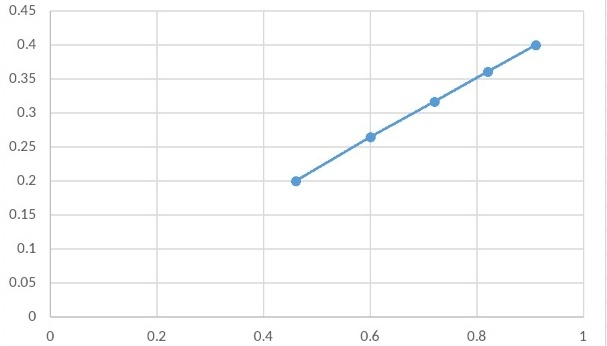
\includegraphics[width=8cm]{Images/min_iv.jpeg}
		\caption{Gráfica $T$ vs $\sqrt{m}$}\label{Fig:min}
	\end{figure}
	\item ¿Qué entiende por MAS?, De los resultados  de la práctica determine la ecuación de movimiento en cada caso.%\cite{ref_05}
	\[x(t)=A\cos(\omega t+ \phi)\]
	\item De acuerdo  a los resultados del experiemnto ¿Cúal es la relación del periodo al variar la masa del péndulo?\\
	No varia, en la fórmula $T=2\pi \sqrt{\tfrac{l}{g}}$, solo depende de la longitud.
\end{enumerate}

%========================================================================================== 